% This is text associated with the open textbook "Open Electromagnetics"
% See immediately below for author, date
% This work is licensed under the Creative Commons Attribution-ShareAlike 4.0 International License. (CC BY-SA 4.0) 
% To view a copy of the license, visit http://creativecommons.org/licenses/by-sa/4.0/

%ORB TITLE The Electric Generator
%ORB AUTHOR 0        # S.W. Ellingson, Virginia Tech (ellingson@vt.edu)
%ORB DATE 20180807   # yyyymmdd
%ORB ABSTRACT The Electric Generator

\label{m0030_Electric_Generator} % <-- Must match name of this file and module directory name.  Don't mess with this!
\index{generator|(}

A generator is a device that transforms mechanical energy into electrical energy, typically by electromagnetic induction via Faraday's Law (Section~\ref{m0055_Faradays_Law}).
For example, a generator might consist of a gasoline engine that turns a crankshaft to which is attached a system of coils and/or magnets.  This rotation changes the relative orientations of the coils with respect to the magnetic field in a time-varying manner, resulting in a time-varying magnetic flux and subsequently induced electric potential.
In this case, the induced potential is said to be a form of \emph{motional emf}, 
\index{emf!motional}
as it is due entirely to changes in geometry as opposed to changes in the magnitude of the magnetic field.
Coal- and steam-fired generators, hydroelectric generators, wind turbines, and other energy generation devices operate using essentially this principle.

Figure~\ref{m0030_fGen} shows a rudimentary generator, which serves as to illustrate the relevant points.
This generator consists of a planar loop that rotates around the $z$ axis; therefore, the rotation can be parameterized in $\phi$.
In this case, the direction of rotation is specified to be in the $+\phi$ direction.
The frequency of rotation is $f_0$; that is, the time required for the loop to make one complete revolution is $1/f_0$.
We assume a time-invariant and spatially-uniform magnetic flux density ${\bf B}=\hat{\bf b}B_0$ where $\hat{\bf b}$ and $B_0$ are both constants.
For illustration purposes, the loop is indicated to be circular. 
However, because the magnetic field is time-invariant and spatially-uniform, the specific shape of the loop is not important, as we shall see in a moment.  Only the area of the loop will matter.
%
\begin{figure}
\begin{center}
\pdftooltip{{  % note double braces
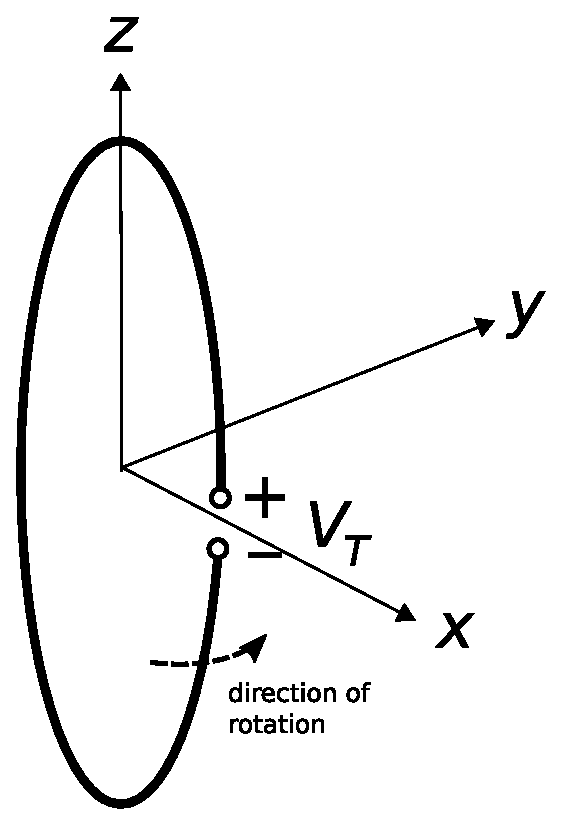
\includegraphics[width=2in]{modules/m0030_fGen.eps}
% ***WikipediaCommonsURL
}}{A single loop generator lying on a three dimensional Cartesian coordinate system, with the z-axis pointed up. On the loop on either side of the x-axis has open nodes, the top positive and the bottom negative. It is labeled V sub T. A dashed arrow curves out of the middle of the loop slightly upward, labeled "direction of rotation".}
\end{center} 
%\centerline{\scriptsize 
%\copyright~\hyperref[***_Credit]{author} 
%\href{https://creativecommons.org/licenses/by-sa/4.0/}{CC BY-SA 4.0} 
%} 
\caption{
\label{m0030_fGen}
A rudimentary single-loop generator, shown at time $t=0$.
}
\end{figure}

The induced potential is indicated as $V_T$ with reference polarity as indicated in the figure.
This potential is given by Faraday's Law:
%
\begin{equation}   
V_T = - \frac{\partial}{\partial t} \Phi
\end{equation}
%
Here $\Phi$ is the magnetic flux associated with an open surface $\mathcal{S}$ bounded by the loop:
%
\begin{equation}   
\Phi = \int_{\mathcal{S}} { {\bf B} \cdot d{\bf s} }
\end{equation}
%
As usual, $\mathcal{S}$ can be any surface that intersects all magnetic field lines passing through the loop, and also as usual, the simplest choice is simply the planar area bounded by the loop.
The differential surface element $d{\bf s}$ is $\hat{\bf n}ds$, where $\hat{\bf n}$ is determined by the reference polarity of $V_T$ according to the ``right hand rule'' convention from Stokes' Theorem.
Making substitutions, we have
%
\begin{flalign}   
\Phi &= \int_{\mathcal{S}} { \left(\hat{\bf b}B_0\right) \cdot \left(\hat{\bf n}ds\right) } \nonumber \\
     &= \left[\hat{\bf b}\cdot\hat{\bf n}\right]B_0 \int_{\mathcal{S}} ds  \nonumber \\
     &= \left[\hat{\bf b}\cdot\hat{\bf n}A\right] B_0 
\end{flalign}
%
where $A$ is the area of the loop.

To make headway, an expression for $\hat{\bf n}$ is needed.
The principal difficulty here is that $\hat{\bf n}$ is rotating with the loop, so it is time-varying.
To sort this out, first consider the situation at time $t=0$, which is the moment illustrated in Figure~\ref{m0030_fGen}.
Beginning at the ``$-$'' terminal, we point the thumb of our right hand in the direction that leads to the ``$+$'' terminal by traversing the loop; $\hat{\bf n}$ is then the direction perpendicular to the plane of the loop in which the fingers of our right hand pass through the loop.  
We see that at $t=0$, $\hat{\bf n}=+\hat{\bf y}$.
A bit later, the loop will have rotated by one-fourth of a complete rotation, and at that time $\hat{\bf n}=-\hat{\bf x}$.
This occurs at $t=1/(4f_0)$.
Later still, the loop will have rotated by one-half of a compete rotation, and then $\hat{\bf n}=-\hat{\bf y}$.
This occurs at $t=1/(2f_0)$.
It is apparent that
%
\begin{equation}
\hat{\bf n}(t) = -\hat{\bf x}\sin 2\pi f_0 t +\hat{\bf y}\cos 2\pi f_0 t
\end{equation}
%
as can be confirmed by checking the three special cases identified above.
Now applying Faraday's Law, we find
%
\begin{flalign}
V_T &= - \frac{\partial}{\partial t} \Phi \nonumber \\
    &= - \frac{\partial}{\partial t} \left[\hat{\bf b}\cdot\hat{\bf n}(t)\right]A B_0 \nonumber \\
    &= - \left[\hat{\bf b}\cdot\frac{\partial}{\partial t}\hat{\bf n}(t)\right]A B_0 
\end{flalign}
%
For notational convenience we make the following definition:
%
\begin{equation}
\hat{\bf n}'(t) \triangleq -\frac{1}{2\pi f_0}\frac{\partial}{\partial t}\hat{\bf n}(t)
\label{m0030_eEGrho}
\end{equation}
%
which is simply the time derivative of $\hat{\bf n}$ divided by $2\pi f_0$ so as to retain a unit vector.  The reason for including a change of sign will become apparent in a moment.
Applying this definition, we find
%
\begin{equation}
\hat{\bf n}'(t) = +\hat{\bf x}\cos 2\pi f_0 t +\hat{\bf y}\sin 2\pi f_0 t
\end{equation}
%
Note that this is essentially the definition of the radial basis vector $\hat{\bf \rho}$ from the cylindrical coordinate system (which is why we applied the minus sign in Equation~\ref{m0030_eEGrho}).  
Recognizing this, we write
%
\begin{equation}
\hat{\bf \rho}(t) = +\hat{\bf x}\cos 2\pi f_0 t +\hat{\bf y}\sin 2\pi f_0 t
\end{equation}
%
and finally
%
\begin{equation}   
\boxed{
V_T = +2\pi f_0 A B_0 \hat{\bf b}\cdot\hat{\bf \rho}(t) 
}
\label{m0030_eGen} 
\end{equation}

If the purpose of this device is to generate power, then presumably we would choose the magnetic field to be in a direction that maximizes the maximum value of $\hat{\bf b}\cdot\hat{\bf \rho}(t)$.
Therefore, power is optimized for ${\bf B}$ polarized entirely in some combination of $\hat{\bf x}$ and $\hat{\bf y}$, and with ${\bf B}\cdot\hat{\bf z}=0$. 
Under that constraint, we see that $V_T$ varies sinusoidally with frequency $f_0$ and exhibits peak magnitude 
%
\begin{equation}  
\boxed{ 
\mbox{max}~\left|V_T(t)\right| = 2\pi f_0 A B_0 
}
\end{equation}
%
It's worth noting that the maximum voltage magnitude is achieved when the plane of the loop is parallel to ${\bf B}$; i.e., when $\hat{\bf b}\cdot\hat{\bf n}(t)=0$ so that $\Phi(t)=0$.  Why is that?  Because this is when $\Phi(t)$ is most rapidly increasing or decreasing.
Conversely, when the plane of the loop is perpendicular to ${\bf B}$ (i.e., $\hat{\bf b}\cdot\hat{\bf n}(t)=1$), $\left|\Phi(t)\right|$ is maximum but its time-derivative is zero, so $V_T(t)=0$ at this instant.

%%%%%%%%%%%%%%%%%%%%%%%%%%%%%%%%%%%%%%%%%%%%%%%
%ORB EXAMPLE
~\\ \begin{example} 
\begin{mdframed}[backgroundcolor=brown!20,linecolor=brown!20]\raggedright
Rudimentary electric generator.
\\~\\
The generator in Figure~\ref{m0030_fGen} consists of a circular loop of radius $a=1$~cm rotating at 1000 revolutions per second in a static and spatially-uniform magnetic flux density of 1~mT in the $+\hat{\bf x}$ direction.
What is the induced potential?

{\bf Solution.}
From the problem statement, $f_0=1$~kHz, $B_0=1$~mT, and $\hat{\bf b}=+\hat{\bf x}$.
Therefore $\hat{\bf b}\cdot\hat{\bf \rho}(t)$ $=$ $\hat{\bf x}\cdot\hat{\bf \rho}(t)$ $=$ $\cos 2\pi f_0 t$.
The area of the loop is $A=\pi a^2$.
From Equation~\ref{m0030_eGen} we obtain 
%
\begin{equation}
V_T(t) \cong \left(1.97~\mbox{mV}\right)\cos\left[\left(6.28~\mbox{krad/s}\right)t\right] 
\nonumber
\end{equation}
\end{mdframed}
\end{example}
%%%%%%%%%%%%%%%%%%%%%%%%%%%%%%%%%%%%%%%%%%%%%%%

Finally, we note that it is not really necessary for the loop to rotate in the presence of a magnetic field with constant $\hat{\bf b}$; it works equally well for the loop to be stationary and for $\hat{\bf b}$ to rotate -- in fact, this is essentially the same problem.  In some practical generators, both the potential-generating coils and fields (generated by some combination of magnets and coils) rotate.


{\bf Additional Reading:}
\begin{itemize}
\item ``\href{https://en.wikipedia.org/wiki/Electric_generator}{Electric Generator}'' on Wikipedia.
%\item \href{https://en.wikipedia.org/wiki/Electric_motor}{Electric Motor} on Wikipedia.
\end{itemize}

\index{generator|)}
